\subsection{Lorenz System}
\subsubsection{Problem Formulation}
We remind the reader of the Lorenz ODE system given in equation \ref{eq:lorenz}, which we repeat here:
\begin{equation*}
\begin{aligned}
    \dot{x} &= \sigma (y - x), \\
    \dot{y} &= x (\rho - z) - y, \\
    \dot{z} &= x y - \beta z,
\end{aligned}
\end{equation*}
where the parameters $\sigma$, $\rho$, and $\beta$ are set to 10, 28, and $8/3$, respectively. 
We attempt to reproduce the results of \textcite{Champion_2019}.

Hence, given the generated high-dimensional data generation discussed in \ref{sec:method}, we consider an encoder with layer widths widths $[128, 64, 32, 3]$, and a decoder with layer widths $[3, 32, 64, 128]$, where 128 is the dimension of our high-dimensional data, and 3 is the dimension of our latent-space. 
We consider a loss formulation with regularization, running $10,000$ initial epochs with regularization and sequential least squares thresholding, before running an additional $1,000$ simulations without regularization. 
To optimize our SINDy Autoencoder, we apply \textsc{ADAM} with a learning rate of $10^{-3}$. 
Further specifics about the training parameters can be found in \autoref{table:lorenz}. 

\begin{table}
\caption{Specifications and hyperparameters used for training our Lorenz system.}
\centering
\begin{tabular}{|l|r|}\hline
    Parameter & Value \\
    \hline
    n & $128$\\
    d & $3$\\
    \text{training samples} & $5.12 \times 10^5$ \\
    batch size & $8000$ \\
    activation function & sigmoid \\
    encoder layers widths & [64, 32]\\
    decoder layer width & [32, 64]\\
    learning rate & $10^{-3}$\\
    SINDy library polynomial order & 3\\
    SINDy library include sines & no\\
    $\lambda_1$ & $10^{-4}$\\
    $\lambda_2$ & $0$ \\
    $\lambda_3$ & $10^{-5}$\\
    thresholding frequency & $500$\\
    thresholding value & $0.1$\\
    \hline
\end{tabular}
\label{table:lorenz}
\end{table}

Using these parameters, we trained 10 models with different random seeds, comparing their results. 

\section{Results}

% \begin{figure*}
% \centering
%     \begin{minipage}[b]{.45\textwidth}
%     \centering
%     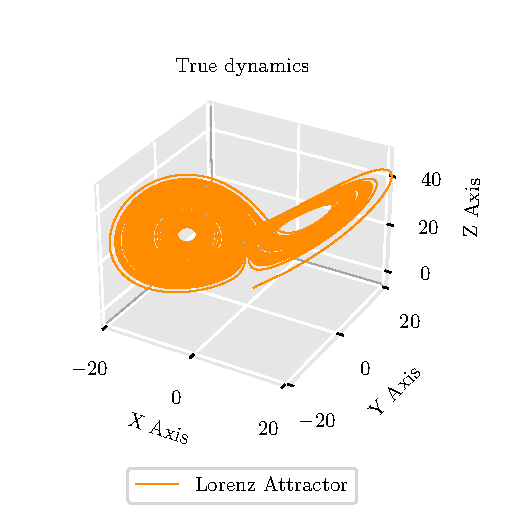
\includegraphics[width=\textwidth]{project_2/images/lorenz_true_dynamics.pdf}
%     \caption{\textbf{.}
%     \label{fig:}
%     \end{minipage}\qquad\quad
%     \begin{minipage}[b]{.45\textwidth}
%     \centering
%     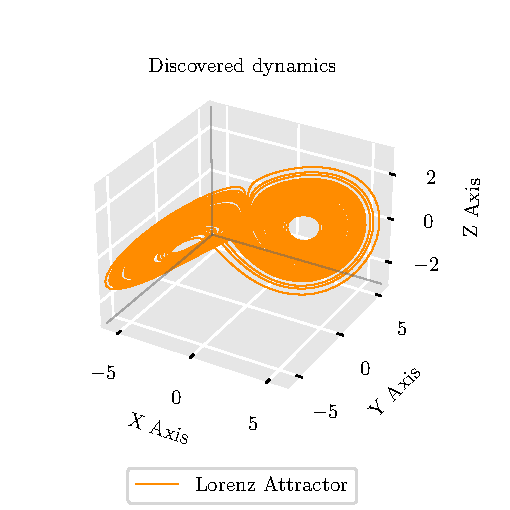
\includegraphics[width=\textwidth]{project_2/images/lorenz_discovered_dynamics.pdf}
%     \caption{\textbf{.}}
%     \label{fig:}
%     \end{minipage}
% \end{figure*}

Using the above formulation, we run 

\subsection{Non-linear Pendulum}
\subsubsection{Problem Formulation}
We again remind the reader of the non-linear pendulumequation given in \ref{eq:pendel}, which is repeated below. 
\begin{equation*}
    \ddot{z} = -\sin(z).
\end{equation*}
Again, we attempt to reproduce the results of \cite{Champion_2019}. The setup specifics for the model are given in \autoref{table:pendulum}. Note that we apply a much smaller batch size 250 compared to Kathleen's 1024. This was primarily done due to excessive memory pressure during our simulations. Also note that since the equation is second order, the SINDy library includes both $z$ and $\dot{z}$ terms, alongside their respective sines. 

\begin{table}
\caption{Specifications and hyperparameters used for training the non-linear pendulum.}
\centering
\begin{tabular}{|l|r|}\hline
    Parameter & Value \\
    \hline
    n & $2601$\\
    d & $1$\\
    \text{training samples} & $5 \times 10^4$ \\
    batch size & $250$ \\
    activation function & sigmoid \\
    encoder layers widths & [128, 64, 32]\\
    decoder layer width & [32, 64, 128]\\
    learning rate & $10^{-4}$\\
    SINDy library polynomial order & 3\\
    SINDy library include sines & yes\\
    $\lambda_1$ & $5 \times 10^{-4}$\\
    $\lambda_2$ & $5 \times 10^{-5}$ \\
    $\lambda_3$ & $10^{-5}$\\
    thresholding frequency & $500$\\
    thresholding value & $0.1$\\
    \hline
\end{tabular}
\label{table:pendulum}
\end{table}

Using these parameters, we trained 7 models with different random seeds, comparing their results. 

\subsubsection{Results}

Should write about computational difference to Lorenz. 